%!TEX root = main.tex

% =============================================================================
\section{System Evaluation}
\label{sec:system-evaluation}
% =============================================================================

Having studied the robust tunings analytically, we are now in a position to test
    our approach with a deployment in a full-blown LSM-based storage engine.
In this section, we provide the details regarding the integration of {\Endure}
    tunings to RocksDB and the performance benchmarking we followed to collect
    empirical results.

\subsection{Experimental Setup \& Implementation}

Our server is powered by two Intel Xeon Gold 6230 processors and has 384 GB 
    of main memory alongside a 1 TB Dell P4510 NVMe drive.
It runs CentOS 7.9.2009 with a default page size of 4 KB.
We use Facebook's RocksDB database, a popular LSM tree-based storage system, to
    evaluate our approach \cite{FacebookMyRocks}.
We use RocksDB's event hooks to implement both classical leveling and tiering
    policies despite its limited support for pure tiering compaction policy
    \cite{RocksDB2020a}.
Following the Monkey memory allocation scheme~\cite{Dayan2017}, we allocate different
    bits per element for Bloom filters per level using the built-in 
    implementation of RocksDB.

\begin{figure*}[ht]
    \centering
    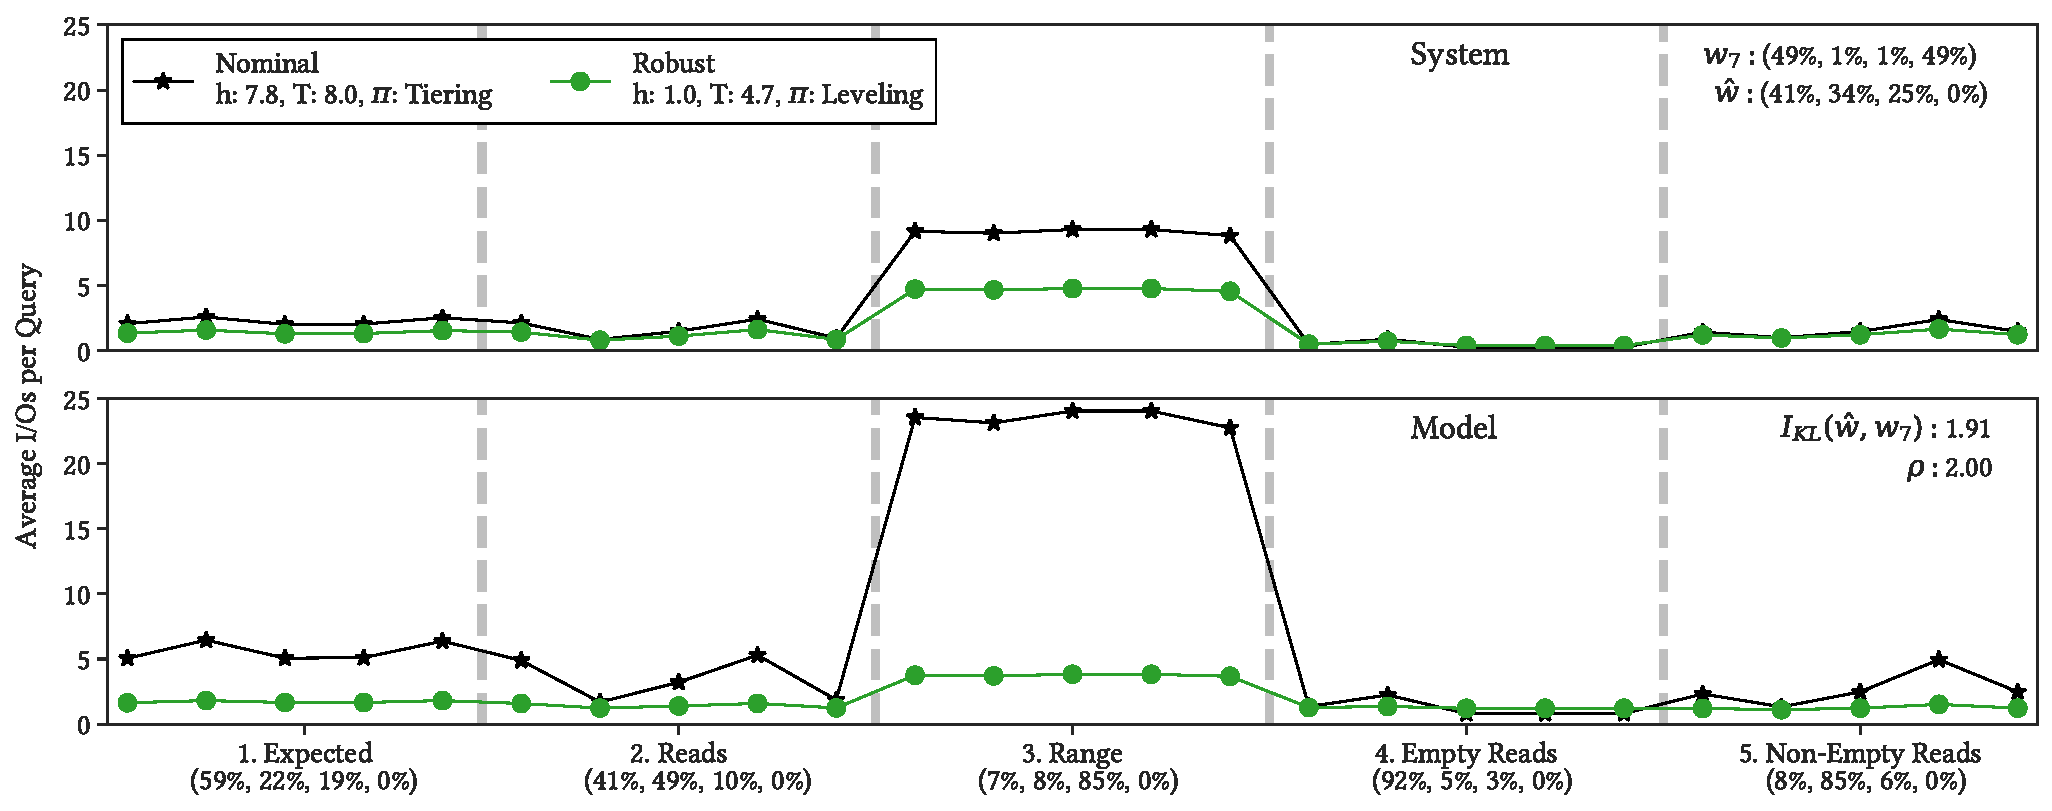
\includegraphics[scale=0.5]{figures/query_seq_read_2.pdf}
    \caption{System (top) and model (bottom) performance for robust and nominal
        tunings in a read-only query sequence. Here the tuning parameter $\rho$
        closely matches the observed value of $I_{KL}(\obsworkload,
        \workload_{7})$.
    Each session contains the label and average workload.
    }
    \label{fig:query_seq_reads_2}
\end{figure*}

\begin{figure*}[ht]
    \centering
    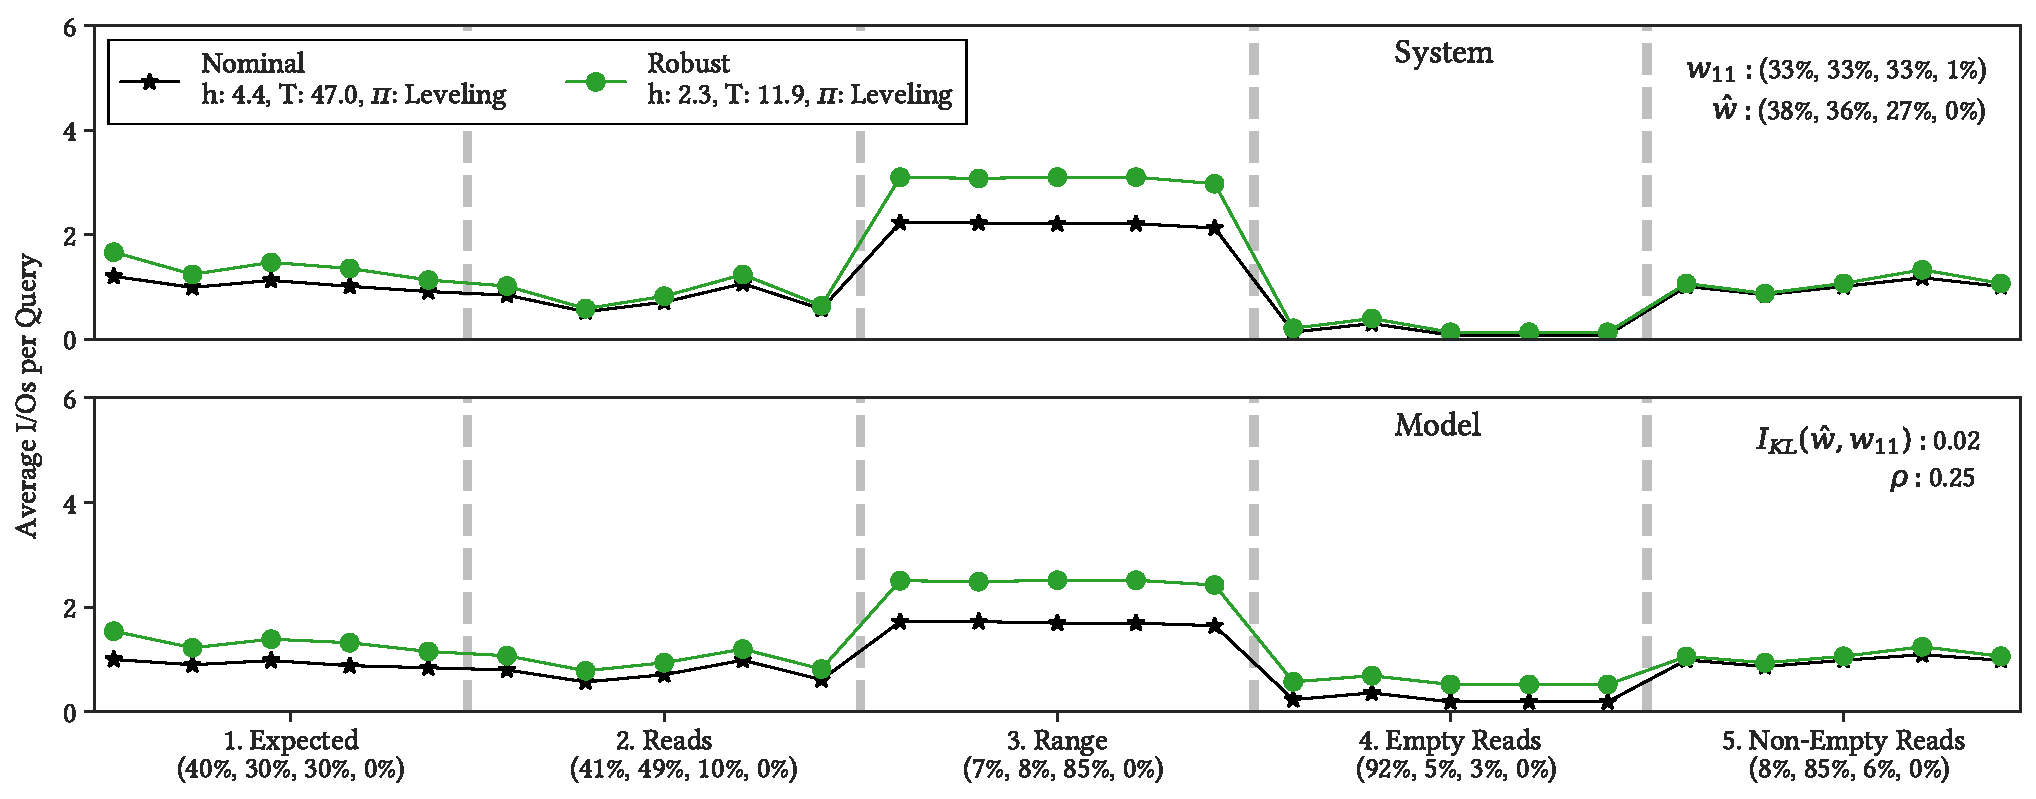
\includegraphics[scale=0.5]{figures/query_seq_read_1.pdf}
    \caption{Read-only query sequence when the observed workloads {\obsworkload}
        do not deviate from the expected.
    }
    \label{fig:query_seq_reads_1}
\end{figure*}

\subsection{Experiment Design}

To evaluate the performance of our proposed robust tuning approach, we create
    multiple instances of RocksDB using different tunings and empirically
    measure their performance while executing workloads from the uncertainty
    benchmark {\benchmark}.
To measure the steady-state performance of the database, each instantiation is
    initially bulk loaded with the exact same sequence of 10 million
    entries each of size 1 KB.
Each key-value entry has a 16-bit uniformly at random 
    sampled key, with the remaining bits being allocated to a randomly 
    generated value.

While evaluating the performance of the database, we sample a sequence of 
    workloads from the benchmark set {\benchmark}.
Each sequence is cataloged into one of the categories — \emph{expected}, 
    \emph{empty read}, \emph{non-empty read}, \emph{read}, \emph{range}, 
    and \emph{write} — based on the dominant query type in the workloads
    in the sequence.
Specifically, the \emph{expected} session contains workloads with a
    KL-divergence less than 0.2 w.r.t. the expected workload used for tuning. 
In all other sessions, the dominant query type encompasses 80\% of the total
    queries in the session.
The remaining 20\% of queries may belong to any of the query types.
While generating actual queries to run on the database, we ensure that non-empty
    point reads query a key that exists in the database, while the empty
    point reads query a key that is not present in the database, but is sampled
    from the same domain.
All range queries are generated with minimal selectivity $S_{RQ}$ to act as 
    short range queries, essentially reading zero or one page per level.
While generating actual short-range queries, we randomly select a sequence of 
    size $B$ (number of entries that fit in a page) from the existing keys. 
Lastly, write queries consist of randomly generated key-value pairs, 
    and thus they may update existing keys already present 
    in the database.

\begin{figure*}[h]
    \centering
    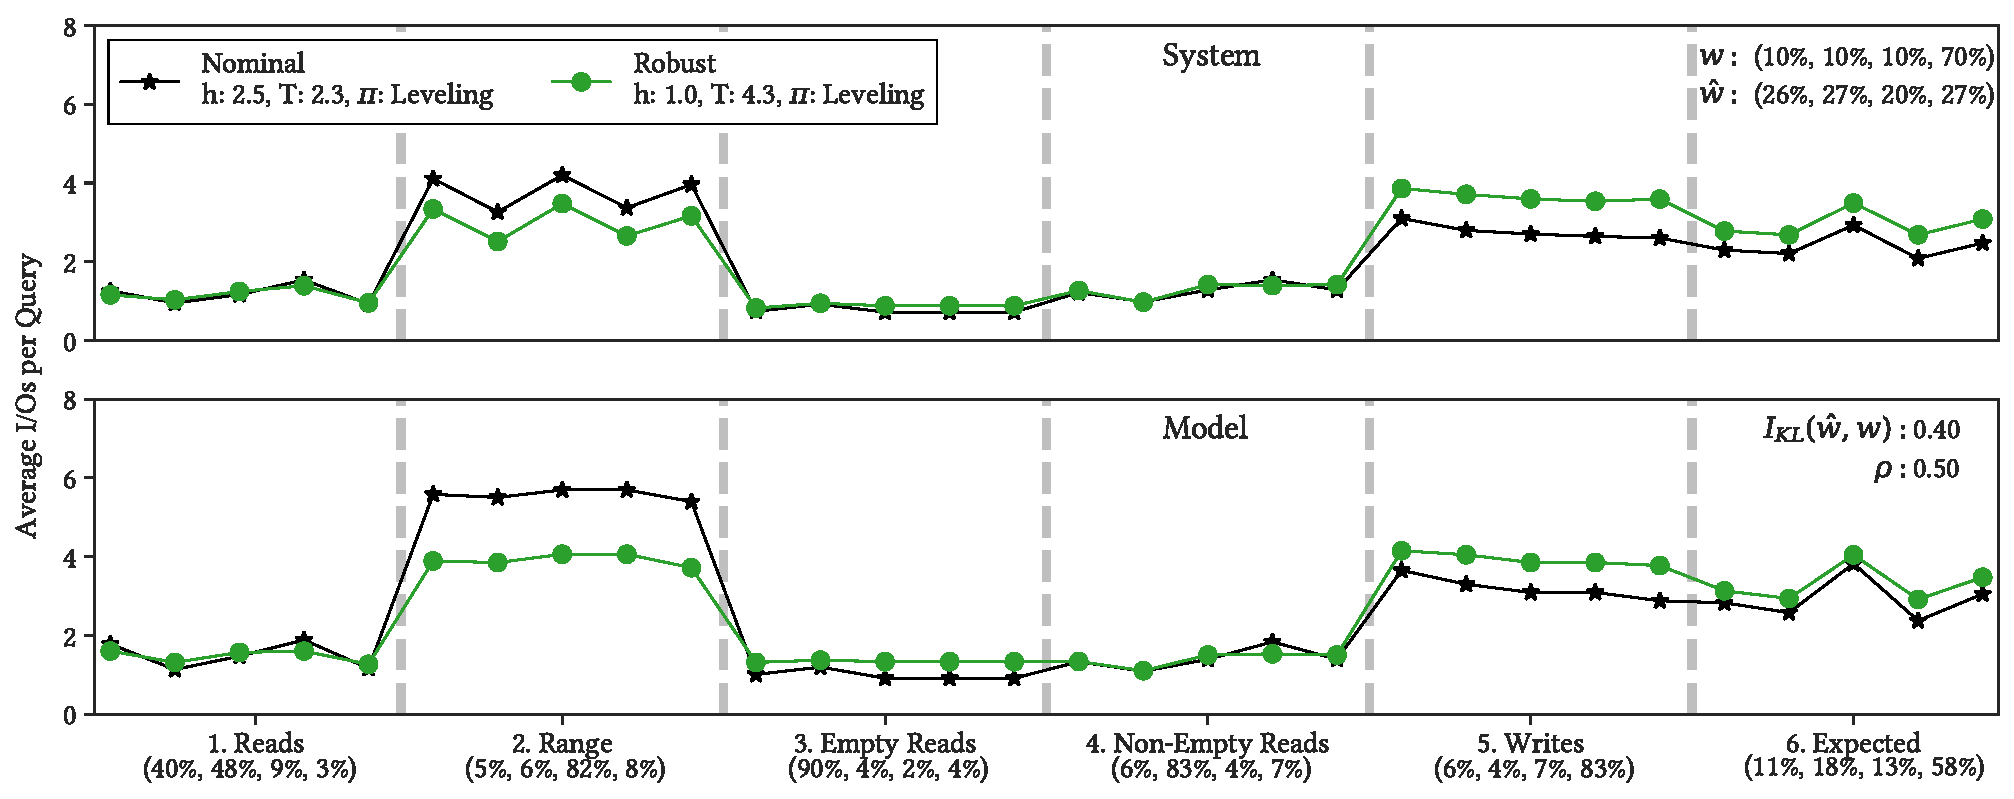
\includegraphics[scale=0.5]{figures/query_seq_hybrid_1.pdf}
    \caption{Read and write workload sequence where $\rho$ and
        $I_{KL}(\obsworkload, \workload)$ closely match.}
    \label{fig:query_seq_hybrid_1}
\end{figure*}

\begin{figure*}[h]
    \centering
    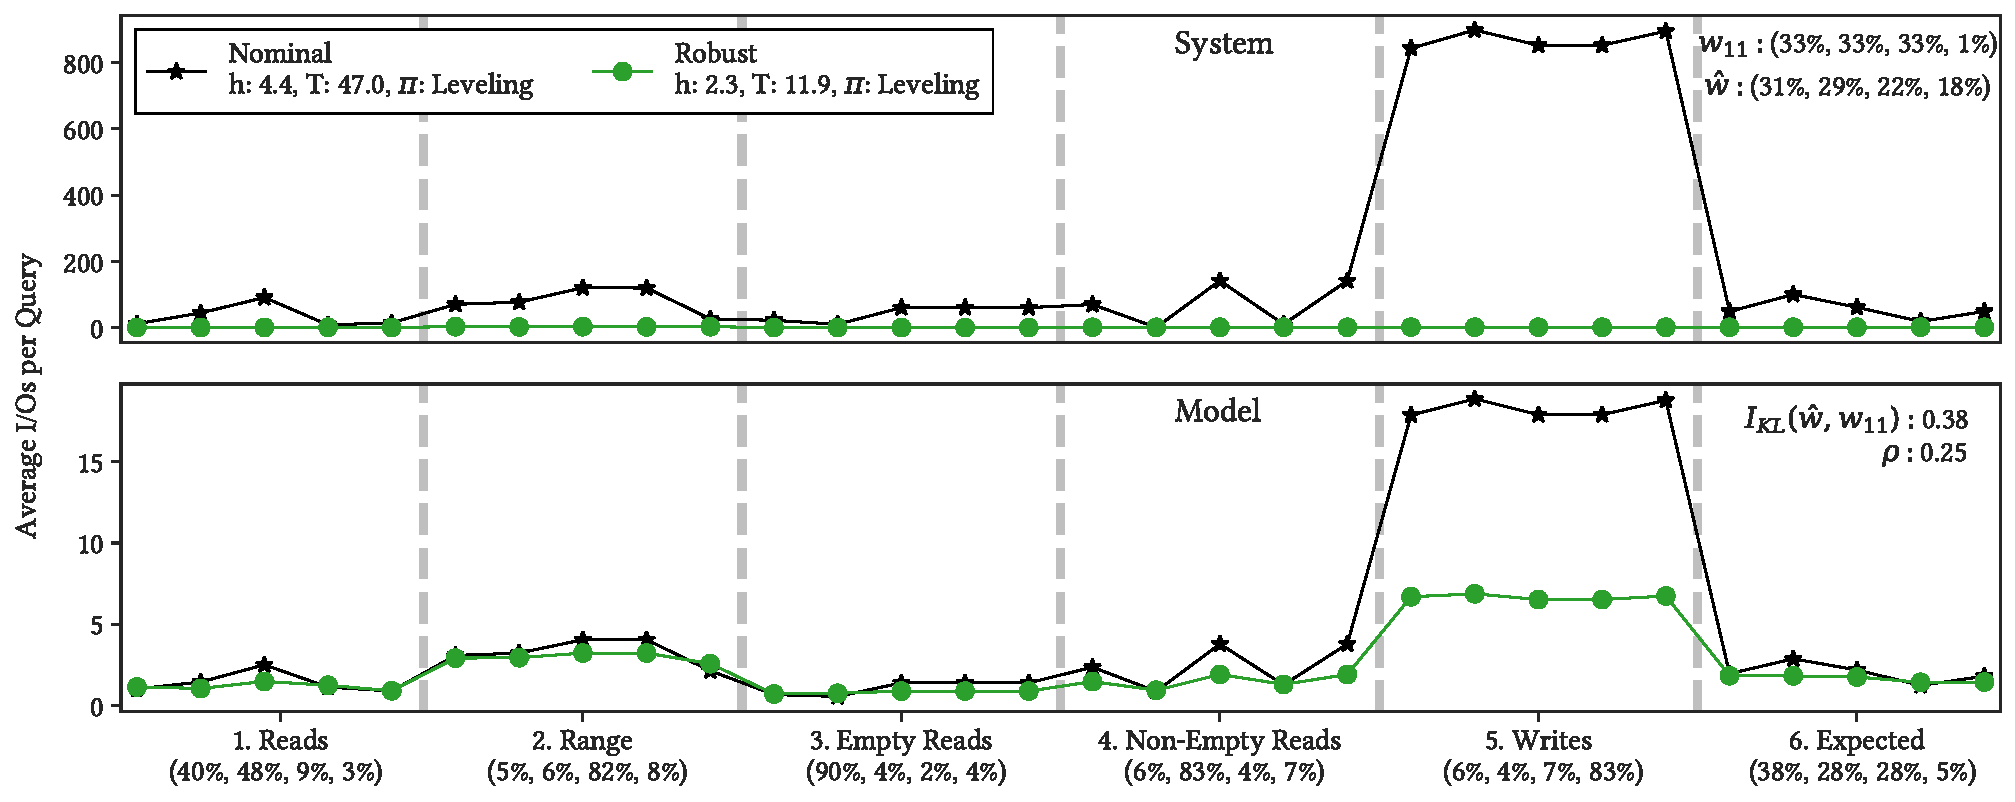
\includegraphics[scale=0.5]{figures/query_seq_hybrid_2.pdf}
    \caption{Read and write workload sequence where $\rho$ and
        $I_{KL}(\obsworkload, \workload)$ closely match.}
    \label{fig:query_seq_hybrid_2}
\end{figure*}


\subsection{Empirical Measurements}
\label{sec:empirical_measurements}
We now provide details about the precise empirical measurements
    during the execution of workloads on RocksDB.
To obtain an accurate count of block accesses in our experiments, 
    we turn off the block cache of RocksDB, and enable direct I/Os for 
    all reads.
We use the internal RocksDB statistics module to measure number of logical block
    accesses during reads, bytes written or flushed during writes, and bytes
    read and written during compactions.
The number of logical blocks accessed during writes is then calculated by 
    dividing the number of bytes reported by the default page size.
It should be noted that precise measurement of write cost is difficult as writes
    inherently change the structure of the database, thereby affecting costs
    associated with all future queries.
To estimate the amortized cost of writes, we compute I/Os from compactions 
    across all workloads of a session and redistribute them across write queries.
Our approach of measuring average I/Os per query allows us to compare the
    effects of different tuning configurations, while simultaneously minimizing
    the effects of extraneous factors on the database performance.


\subsection{Results}
\label{sec:system-results}

We first validate the analytical model discussed in
    Section~\ref{sec:tuning_lsm_trees} and then
    replicate key insights from Section~\ref{sec:model-evaluation} on a 
    RocksDB database.
In our implementation, the instantiation of RocksDB database combined with bulk loading
    requires on an average 10 minutes, while individual workloads are executed
    in about 3 minutes on an average.

\Paragraph{Read Performance Validation}
As discussed earlier in Section~\ref{sec:empirical_measurements}, write queries
    change the structure of the LSM tree and affect the costs of all following
    queries.
Hence, we begin by first validating the accuracy of the analytical model for read queries in
    Figures~\ref{fig:query_seq_reads_2} and~\ref{fig:query_seq_reads_1}
    which exclude write sessions.
In both figures, we compare actual I/Os per query on the database system (top)
    with the I/Os per query predicted by the model (bottom) for both nominal and 
    robust tunings across different read session.
We observe that the empirical measurements not only confirm the cost model 
    predictions but also provide evidence in support of relative performance
    between different tunings.
The discrepancy observed between the relative performances between the nominal
    and the robust tunings in the presence of range queries is due to the fence pointers in RocksDB.
The analytical model does not account for the fence pointers which reduce the 
    measured I/Os for (some) short range queries, thereby increasing the predicted I/Os. 

\Paragraph{Write Performance Validation}
Now, we validate the write-portion of the analytical model by introducing an additional write 
    query dominated session in Figures~\ref{fig:query_seq_hybrid_1} and 
    ~\ref{fig:query_seq_hybrid_2}.
Note that the structure of the LSM tree is continually changing across all the
    session in these figures due to the compactions caused by the write queries.
For example, the dips in measured I/Os in the range query session in Figure
    ~\ref{fig:query_seq_hybrid_1} are the result of compactions triggered
    by write queries in preceding workloads leading to empty levels.
Moreover, in Figure~\ref{fig:query_seq_hybrid_2}, the large size-ratio {\sizeratio}
    leads to a shallow tree with extremely large levels. 
Thus, a compaction occurring in the write query dominated session triggers a sort
    at the lower levels of the tree resulting in a higher number of I/Os than
    predicted by the model. 
Overall, Figures~\ref{fig:query_seq_reads_2}--~\ref{fig:query_seq_hybrid_1} confirm
    that our analytical model can accurately capture the relative 
    performance of different tunings.

\Paragraph{Choice of Tuning Parameter $\rho$ Validation}
In the model evaluation (Figure~\ref{fig:rho_vs_rho_hat} in Section
    \ref{sec:model-results}), we showed that robust tuning outperforms the
    nominal tuning in the presence of uncertainty for tuning parameter $\rho$
    approximately greater than 0.2.
This is further supported by all the system validation experiments described
    above.
Specifically, Figures~\ref{fig:query_seq_reads_2}, ~\ref{fig:query_seq_hybrid_1},
    and~\ref{fig:query_seq_hybrid_2} show instances where the KL-divergence
    of the observed workload averaged across all the sessions w.r.t. the expected
    workload is close to the tuning parameter $\rho$.
In each of these experiments, the robust tuning outperforms the nominal.
Conversely, in Figure~\ref{fig:query_seq_reads_1}, we find that the observed
    workloads are very similar to the expected workload ($I_{KL}(\obsworkload,
    \workload_{11}) = 0.2$), resulting in a performance benefit in favor of the
    nominal tuning, as predicted in Figure~\ref{fig:rho_vs_rho_hat}.

\subsection{Robustness is All You Need}

One of the key challenges during the evaluation of tuning configurations in 
    presence of uncertainty is the challenge in measuring a steady-state
    performance.
In Section~\ref{sec:system-results}, we show that the cost-model can accurately
    predict the empirical measurements.
In the course of this study, using our model, we compared over 700 different
    robust tunings with their nominal counterparts over the uncertainty
    benchmark set {\benchmark}, leading to approximately 8.6 million
    comparisons.
Robust tunings comprehensively outperform the nominal tunings in over 80\% of
    these comparisons.
We further cross-validated the relative performance of the nominal and the 
    robust tunings in over 300 of these comparisons using RocksDB.
The empirical measurements overwhelmingly confirmed the validity of our 
    analytical models, and the few instances of discrepancy in the scale of 
    measured I/Os, such as the ones discussed in previous section, are 
    easily explained based on the structure of the LSM tree.
    
One of the key takeaways of applying robust tuning to LSM trees is that
    \emph{the leveling policies are inherently more robust} to perturbations in
    workloads, when compared to pure tiering policies.
This observation is in line with the industry practice of deploying leveling or
    hybrid policies over pure tiering policies.
Overall, based on our analytical and empirical results, robust tuning should
    always be employed when tuning an LSM tree to obtain robust tuning
    configurations, unless the future workload distribution is known with
    absolute certainty.

\Paragraph{Discussion}
While we have deployed and tested robust tuning on LSM trees, the robust
    paradigm of {\Endure} is a generalization of a minimization problem which is
    at the heart of any database tuning problem.
Hence, similar robust optimization approaches can be applied to \emph{any
    database tuning} problem assuming that the underlying cost-model is known,
    and each cost-model component is convex or can be accurately approximated by
    a convex surrogate. 

% =============================================================================
